\documentclass[a4paper,12pt]{article}
\usepackage[catalan]{varioref}
\usepackage{setspace}
\usepackage[margin=2.54cm]{geometry}
\usepackage{pdfpages}
\usepackage[utf8]{inputenc}
\usepackage[catalan]{babel}
\usepackage{graphicx,subcaption}
\usepackage{graphics}
\usepackage{lscape}
\usepackage{pdflscape}
\usepackage{float}
\usepackage{textcomp}
\usepackage{amsmath}
\usepackage{hyperref}
\usepackage{fancyvrb}
\usepackage{parskip}
\usepackage{changepage}
\usepackage{enumitem}
\usepackage{tcolorbox}
\usepackage[all]{hypcap}
\usepackage{xcolor}
\usepackage{listings}
\usepackage[hidelinks]{hyperref}
\definecolor{green}{HTML}{228B22}
\definecolor{orange}{HTML}{FFC107}
\usepackage{color}
\definecolor{dkgreen}{rgb}{0,0.6,0}
\definecolor{gray}{rgb}{0.5,0.5,0.5}
\definecolor{mauve}{rgb}{0.58,0,0.82}
\lstset{escapeinside={<@}{@>}}

\hypersetup{
    colorlinks,
    citecolor=black,
    filecolor=black,
    linkcolor=black,
    urlcolor=black
}


\lstset{frame=tb,
    language=java,
    aboveskip=3mm,
    belowskip=3mm,
    showstringspaces=false,
    columns=flexible,
    basicstyle={\small\ttfamily},
    numbers=none,
    numberstyle=\tiny\color{gray},
    keywordstyle=\color{blue},
    commentstyle=\color{dkgreen},
    stringstyle=\color{mauve},
    breaklines=true,
    breakatwhitespace=true, tabsize=3
}
\title{
	\begin{center}
	\vspace{3cm}
	\includegraphics[width=11cm, height=3cm]{images/Logo-nou-eps.jpg}
	\end{center}
	\begin{center}
	\line(1,0){340}
	\end{center}		
	AMPLIACIÓ DE BASES DE DADES I ENGINYERIA DEL PROGRAMARI\\
	\vspace{2mm}
	\Large Pràctica 3: Primera activitat de patrons de disseny\\
	\line(1,0){340}
	\vspace{2.5cm}
	}

\author{Aaron Arenas Tomas - 78098697N \\ Ramon Escoda Semís - 49751728Z \\   Marc Cervera Rosell - 47980320C \vspace{1cm}}


\date{18 de maig 2022\vspace{0.5cm} \\Grau en Enginyeria Informàtica}
\onehalfspacing

\begin{document}
	\begin{titlepage}
		\maketitle
		\thispagestyle{empty}
	\end{titlepage}
	\cleardoublepage
	\newpage

\tableofcontents
\listoffigures
\thispagestyle{empty}

\newpage
\section{Disseny}

\begin{figure}[H]
    \centering
    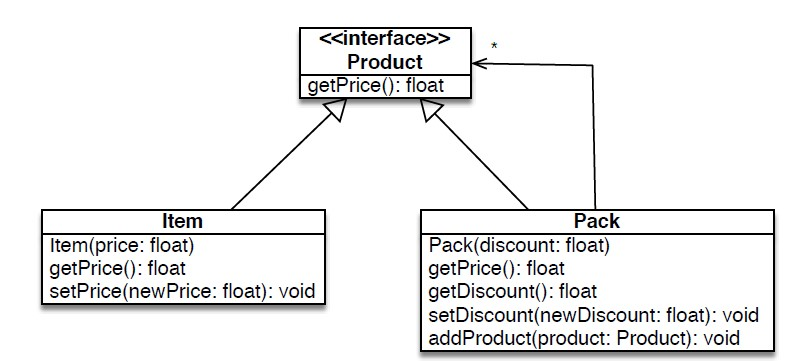
\includegraphics[scale = 0.7]{images/uml.jpg}
    \caption{Disseny UML}
    \label{fig:UML}
\end{figure}

\justify{Especificacions dels mètodes de les classes: \\}

\begin{figure}[H]
    \centering
    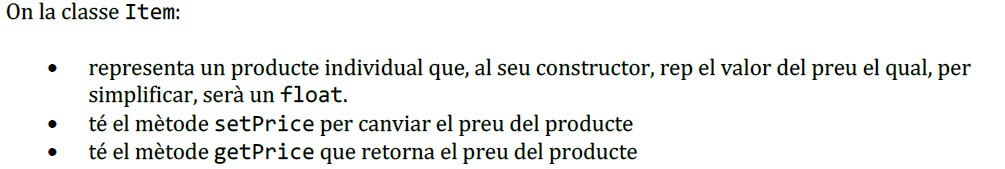
\includegraphics[scale = 0.6]{images/classe item.jpg}
    \caption{Especificacions dels mètodes de la classe \textit{Item}}
    \label{fig:Item}
\end{figure}

\begin{figure}[H]
    \centering
    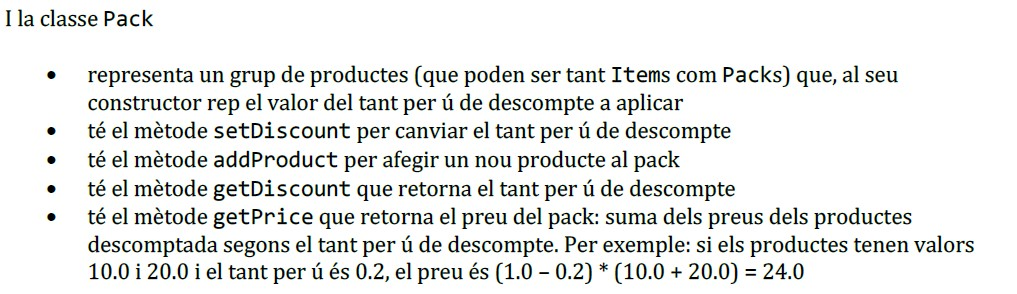
\includegraphics[scale = 0.6]{images/classe pack.jpg}
    \caption{Especificacions dels mètodes de la classe \textit{Pack}}
    \label{fig:Pack}
\end{figure}

\begin{figure}[H]
    \centering
    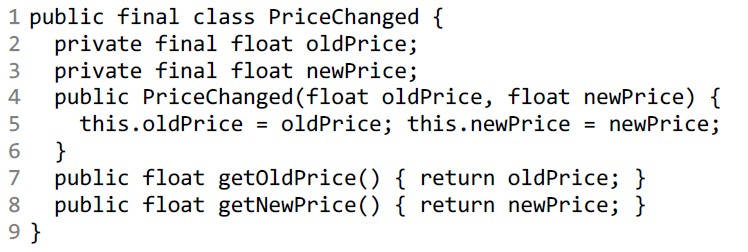
\includegraphics[scale = 0.7]{images/classe PriceChanged.jpg}
    \caption{Especificacions dels mètodes de la classe \textit{PriceChanged}}
    \label{fig:PriceChanged}
\end{figure}

\pagenumbering{arabic}
\section{Solució consensuada}
\justify{Un cop comparades totes les resolucions individuals, les quals s'adjunten juntament amb aquest document, s'ha decidit, per unanimitat, entregar com a solució vàlida (segons el critèri dels membres del grup) i puntuable, la solució que s'observa a continuació.\\
Com es podrà observar, en el codi de la solució final hi ha mètodes que no formen part de la solució al problema demanat, però s'han inclòs atès que s'ha usat l'IDE per programar la totalitat del codi i s'ha fet ús d'una classe anomenada \textit{Main} que realitza diversos jocs de proves per comprovar la correctesa de la solució. Per poder veure la classe \textit{Main}, hi ha dues opcions; veure l'annex d'aquest document (Secció \textit{\vref{sec:Annex}}) o seguir l'enllaç al directori de GitHub que hi ha més andavant (Secció \textit{\vref{sec:link}}).}

\subsection{Classe abstracta \textit{Product}}

\begin{lstlisting}
/* 
   Marc Cervera Rossell
   Aaron Arenas Tomas
   Ramon Escoda Semis
*/

public abstract class Product extends Observable {
    public abstract float getPrice();
}

\end{lstlisting}
\newpage
\subsection{Classe \textit{Item}}
\begin{lstlisting} 
/* 
   Marc Cervera Rossell
   Aaron Arenas Tomas
   Ramon Escoda Semis
*/

public class Item extends Product {
    private float price;

    public Item(float price) {
        this.price = price;
    }

    @Override
    public float getPrice() {
        return this.price;
    }

    public void setPrice(float price) {
        if (price < 0) {
            throw new IllegalArgumentException("Negative price");
        }
        if (this.price != price) {
            float oldP = this.price;
            this.price = price;
            notifyObservers(new PriceChanged(oldP, this.price));
        }
    }

    @Override
    public String toString() {
        return "Item {" +
                "price = " + price +
                '}';
    }
}
\end{lstlisting}
\newpage
\subsection{Classe \textit{Pack}}
\begin{lstlisting}
/* 
   Marc Cervera Rossell
   Aaron Arenas Tomas
   Ramon Escoda Semis
*/

public class Pack extends Product implements Observer {

    private float discount;

    private boolean hasChanged;

    private float price;

    private List<Product> products;

    public Pack(float discount) {
        this.discount = discount;
        this.products = new ArrayList<Product>();
        this.hasChanged = false;
    }

    public void removeProd(Product p) {
        this.products.remove(p);
    }

    @Override
    public float getPrice() {
        if (!this.hasChanged) {
            return this.price * (1f - getDiscount());
        }
        for (Product p : products) {
            this.price += p.getPrice();
        }
        this.hasChanged = false;
        return this.price * (1f - getDiscount());
    }

    public float getDiscount() {
        return discount;
    }

    public void setDiscount(float discount) {
        if (discount < 0f || discount > 1f) {
            throw new IllegalArgumentException("Not valid discount");
        }
        if (this.discount != discount) {
            float olD = this.discount;
            this.discount = discount;

        }
    }

    public void addProduct(Product product) {
        this.products.add(product);
        float oldP = this.price;
        product.addObserver((Observer) this);
        this.price += product.getPrice();
        notifyObservers(new PriceChanged(oldP, this.price));
    }

    @Override
    public String toString() {
        return "Pack {" +
                "discount = " + discount +
                ", products = " + products +
                '}';
    }

    @Override
    public void update(Observable o, Object arg) {
        PriceChanged pC = (PriceChanged) arg;
        float oldP = this.price;
        if (pC.getNewPrice() != pC.getOldPrice()) {
            this.hasChanged = true;
            notifyObservers(new PriceChanged(oldP, this.getPrice()));
        }
    }
}

\end{lstlisting}
\newpage
\subsection{Classe \textit{PriceChanged}}
\begin{lstlisting}
/* 
   Marc Cervera Rossell
   Aaron Arenas Tomas
   Ramon Escoda Semis
*/

public final class PriceChanged {
    private final float oldPrice;
    private final float newPrice;

    public PriceChanged(float oldPrice, float newPrice) {
        this.oldPrice = oldPrice;
        this.newPrice = newPrice;
    }

    public float getOldPrice() {
        return oldPrice;
    }

    public float getNewPrice() {
        return newPrice;
    }
}


\end{lstlisting}

\subsection{Interfície \textit{Observer}}
\begin{lstlisting}
public interface Observer {
/* 
   Marc Cervera Rossell
   Aaron Arenas Tomas
   Ramon Escoda Semis
*/

    void update(Observable o, Object arg);
}
\end{lstlisting}

\section{Enllaç al directori GitHub}\label{sec:link}
\justify{En aquesta secció és troba l'enllaç al directori de GitHub amb el codi de la solució final. Com es podrà observar, el projecte d'IntellIJ disposa d'una classe \textit{Main}, on hi ha diferets exemples d'execució on es comprova la correctesa dels diferents patrons aplicats.\\}
\href{https://github.com/marc7666/3rd_practical_case_Software_engineering_II.git}{\textbf{\textit{Enllaç al directori GitHub}}}

\section{Annex}\label{sec:Annex}
\subsection{Classe \textit{Main}}
\justify{Com s'ha esmentat en anterioritat en aquest document, aquesta classe ha servit a l'equip de desenvolupament per ratificar la correctesa de la solució que s'ha donat com a vàlida per ésser puntuable.}
\subsubsection{Codi de la classe \textit{Main}}
\begin{lstlisting}
public class Main {
/* 
   Marc Cervera Rossell
   Aaron Arenas Tomas
   Ramon Escoda Semis
*/

    public class Main {
    public static void main(String[] args) {
        /* Pack */
        Pack p1 = new Pack(0.5f);

        /* Items */
        Item i1 = new Item(12.7f);
        Item i2 = new Item(10.13f);
        Item i3 = new Item(400.99f);

        /* Including items inside the pack */
        p1.addProduct(i1);
        p1.addProduct(i2);
        p1.addProduct(i3);

        System.out.println("---------- Composite pattern test part ----------");
        System.out.println("\n");
        System.out.println("---------- Pack with items ----------");
        System.out.println(p1);
        System.out.println("Final price after discount: " + (p1.getPrice()));

        /* Adding a pack inside a pack */
        Pack p2 = new Pack(0.1f);
        Item i4 = new Item(1.7f);
        Item i5 = new Item(123.45f);
        p2.addProduct(i4);
        p2.addProduct(i5);
        p1.addProduct(p2);

        System.out.println("\n");

        System.out.println("---------- Adding a pack inside a pack ----------");
        System.out.println(p1);
        System.out.println("Final price after discount: " + (p1.getPrice()));

        System.out.println("\n");

        System.out.println("---------- Observer test part ----------");
        /* Pack */
        Pack p3 = new Pack(0.6f);

        /* Items */
        Item i6 = new Item(121.7f);
        Item i7 = new Item(105.13f);
        Item i8 = new Item(4000.99f);

        p3.addProduct(i6);
        p3.addProduct(i7);
        p3.addProduct(i8);

        System.out.println(p3);
        i6.setPrice(120.45f);
        System.out.println(i6.getPrice());
        System.out.println(p3);

    }
}
\end{lstlisting}


\end{document}

